
  % Quine quotation.

  This chapter will describe an implementation of \algo which uses
  Nested Data Parallelism in Haskell (by \cite{Harness2008}).
  First, a a few predefined functions will be presented to
  increase their the understanding of their operational behavior.
  Then the implementation will be presented and it's complexities will
  calculated.
  
  \section{Approach}
  
    \subsection{Scanl}
      Parallel prefix sum has well studied efficient implementaitons. One of them
      is the following:
      \begin{lstlisting}   
scanlP f z xs =
  joinD
    . mapD (\(as,a) -> mapS (f a) as)
    . propagateD f z
    . mapD (scanlS f z)
    . splitD
    $ xs
      \end{lstlisting}
      This implementatin is designed to reduce communication
      and therefor increase efficiency. It works in three steps.
      First, each PU computes its local prefix sum (line 5).
      Second, the total sum of each of the PUs is propagated
      around adding up subsequent values.
      Third, the updated sum is used to increase the values of the local chunks.
      This approach is visualised in \ref{figure:scanlPsteps}
      
      \begin{figure}[h!]
          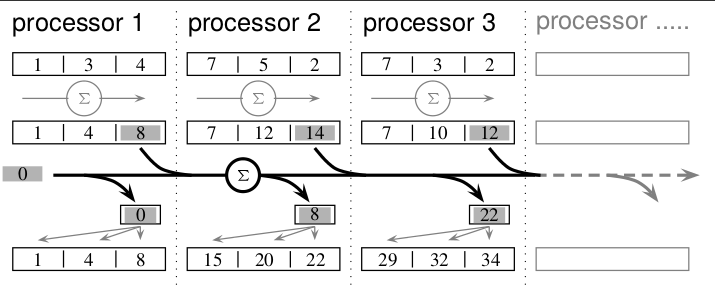
\includegraphics[width=\linewidth]{scanlP-three-steps.png}
          \caption{Parallel prefix sum in three steps (Figure from \cite{DistTypes1999}) }
          \label{figure:scanlPsteps}
      \end{figure}
      The propagation is the bottle neck in terms of dpeth and parallel complexity.
      But since the progapation itself is structurally isomorphic to prefix the entire sum,
      we can use a more efficient scheme for propagation - rather than using linear propagation.
      Propagation in logarithmic depth is possible and an be derived from \cite{Scanl1980}.
      For our purposes, it is sufficient to know the following complexities for scanlP:
      $\W(n) \in O(n)$ and $\D(n) \in O(\log n)$.

    \subsection{GroupP}
      \c{groupP} is a frequently used function in functional programming.
      Given an array it returns an array of arrays,
      where each subarray contains equal consecutive
      elements of the source array. For example
      \c{groupP [1,2,2,2,2,3,3,4]} becomes \c{[[1],[2,2,2,2],[3,3],[4]]}.
      In NDP, the latter is represented by
      \begin{lstlisting}
      AArr {
        data = [# 1,2,2,2,3,3,4 #],
        segd = ATup2 {
          as = [# 0,1,5,7 #]
          bs = [# 1,4,2,1 #]
        }
      }
      \end{lstlisting}
      The key insight in an efficient parallel implementation of \c{groupP}
      relies on the following insight - the data field in the nested array
      is the source array itself! To implement \c{groupP} we only
      need to efficiently calculate the segment descriptor field. This is
      possible in logarithmic depth of the size of the input array!
      
      \begin{figure}[h!]
          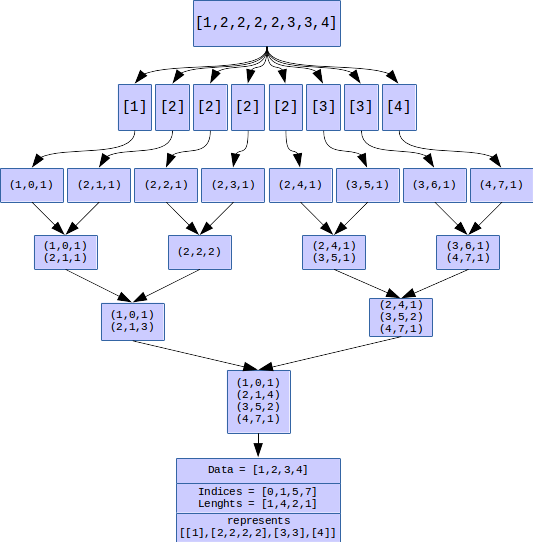
\includegraphics[width=\linewidth]{groupP.png}
          \caption{An example calculation of groupP. Each box is a PU.}
          \label{figure:groupP}
      \end{figure}
      
      As visualised in the figure \ref{figure:groupP}
      we can do that by spliting all elements onto all PUs first.
      Then each PU creates a local chunk of a linked list of
      \c{(Value,StartIdx,Count)}-Triplets to record it singleton.
      After that, each level of recursion merges two PUs by
      merging the last triplet of the left list with the first triplet
      of the right list. If both triplets correspond to the same value,
      then a new triplet with the total count and the left index is used.
      If both are unequal, then they are left unchanged. The implementation
      of \c{groupP} uses a subfunction \c{segdSplitMerge} to implement the
      splitting and merging. This function will be exposed lateron in
      the vectorization of \ndpn.
      Further analysis reveals the complexities $\W(n) \in O(n)$ and $\D(n) \in O(\log n)$.
      All in all, \c{groupP} is an operation which can very well exploit the flat representation of nested arrays.
      
    \subsection{SortP}
      General parallel sorting can be as simple as a parallel
      implementation of merge-sort where the recursive calls are executed
      in parallel. This comparision based sorting has complexities of
      $\W(n) \in O(n \log n)$ and $\D(n) \in O(\log n)$. 
      
  \section{Implementation}
    \begin{lstlisting}
type Image = [:[:Int:]:]
type Hist a = [:a:]

hbalance :: Image -> Image
hbalance img =
    let h = hist img
        a = accu h
        a0 = headP a
        agmax = lastP a
        n = normalize a0 agmax a
        s = scale gmax n
        img' = apply s img
    in  img'

hist :: Image -> Hist Int
hist = sparseToDenseP (gmax+1) 0
          . mapP (\g -> (headP g,lengthP g))
          . groupP
          . sortP
          . concatP

accu :: Hist Int -> Hist Int
accu = scanlP (+) 0

normalize :: Int -> Int -> Hist Int -> Hist Double
normalize a0' agmax' as =
    let a0 = fromIntegral a0'
        agmax = fromIntegral agmax'
        divisor = agmax - a0
    in  [: (fromIntegral freq' - a0) / divisor | freq' <- as :]

scale :: Int -> Hist Double -> Hist Int
scale gmax as = [: floor (a * fromIntegral gmax) |  a <- as :]

apply :: Hist Int -> Image -> Image
apply as img = mapP (mapP (as !:)) img
    \end{lstlisting}
  \section{Complexities}
    ...
    
    % TODO: Genau erläuteren und präzisieren wie Work&Depth mit der Anzahl der Prozessoren in den distributed Types zusammenhängen.
    %    Die tatsächliche Parallelität steck in der Anzahl der PUs (Processing Units) und den verteilten Algorithmen
    %    zwischen den einzelnen PUs. Damit wird sumD und propagateD auf D(log n) gedrückt.
        
    % Ignoriert!! Twofold interpretation: divL = <built-in parallel divL> OR < mapD divS> with distributed types and extended library optimization
    % immer die zweite variante - weil sonst das andere Pman program nicht ginge.
      
    
